\documentclass[12pt]{gruppe-11-article-a5}

\title{Handbuch Editor}
\author{Katharina Böcker, Bill Akhter, David Hamberger, Dennis Authaler, Nick Bethke, Tom Haßler}
\version{alpha 0.1}



\begin{document}
\maketitle
\tableofcontents
\newpage
\hypersetup{
	colorlinks=true,
	linkcolor=linkcolor,
	filecolor=magenta,
	urlcolor=urlcolor,
}


\section{Allgemein}\label{sec:allgemein2}

Dieses Handbuch beschreibt die Funktionsweise des Editors für das Spiel \emph{Battle of the Centerländ}.
\\\\
Der Editor ist in der Programmiersprache \emph{JavaScript}/\emph{TypeScript} und den \emph{Node.js}-Frameworks \emph{Electron} und \emph{React} geschrieben.
\\\\
Der Editor ist in der Lage, die Spielbretter und Spielkonfigurationen zu generieren, zu bearbeiten und zu speichern.
Die Spielbretter und Spielkonfigurationen werden in \emph{JSON}-Dateien gespeichert.
\\\\
Der Editor ist in der Lage, die Spielbretter und Spielkonfigurationen zu validieren.
Die Validierung wird durchgeführt, wenn der Benutzer das Spielbrett oder die Spielkonfiguration bearbeitet.
Die \emph{JSON}-Dateien werden nach den \emph{JSON Schemas} validiert, welche im Standard-Komitee entwickelt wurden.
\\\\
Durch die Implementierung des Editors in \emph{JavaScript}/\emph{TypeScript} und der Verwendung des Framework \emph{Electron}, ist der Editor auf allen gängigen Betriebssystemen lauffähig, da \emph{Electron} auf \emph{Chromium} basiert, welches auf allen gängigen Betriebssystemen verfügbar ist.


\section{Installation}\label{sec:installation}

Abhängig von dem Betriebssystem, auf dem der Editor installiert werden soll, gibt es unterschiedliche Installationsanweisungen.

\subsection{Windows}\label{subsec:windows}

\begin{enumerate}
	\item Laden Sie die Installationsdatei für Windows herunter.
	\item Führen Sie die Installationsdatei aus.
	\item Folgen Sie den Anweisungen des Installationsassistenten.
	\item Nach der Installation ist der Editor über das Startmenü oder über den Desktop erreichbar.
\end{enumerate}

\subsection{Linux}\label{subsec:linux}

\dots

\subsection{macOS}\label{subsec:macos}

\dots


\section{Benutzung}\label{sec:benutzung}

\subsection{Startbildschirm}\label{subsec:startbildschirm}

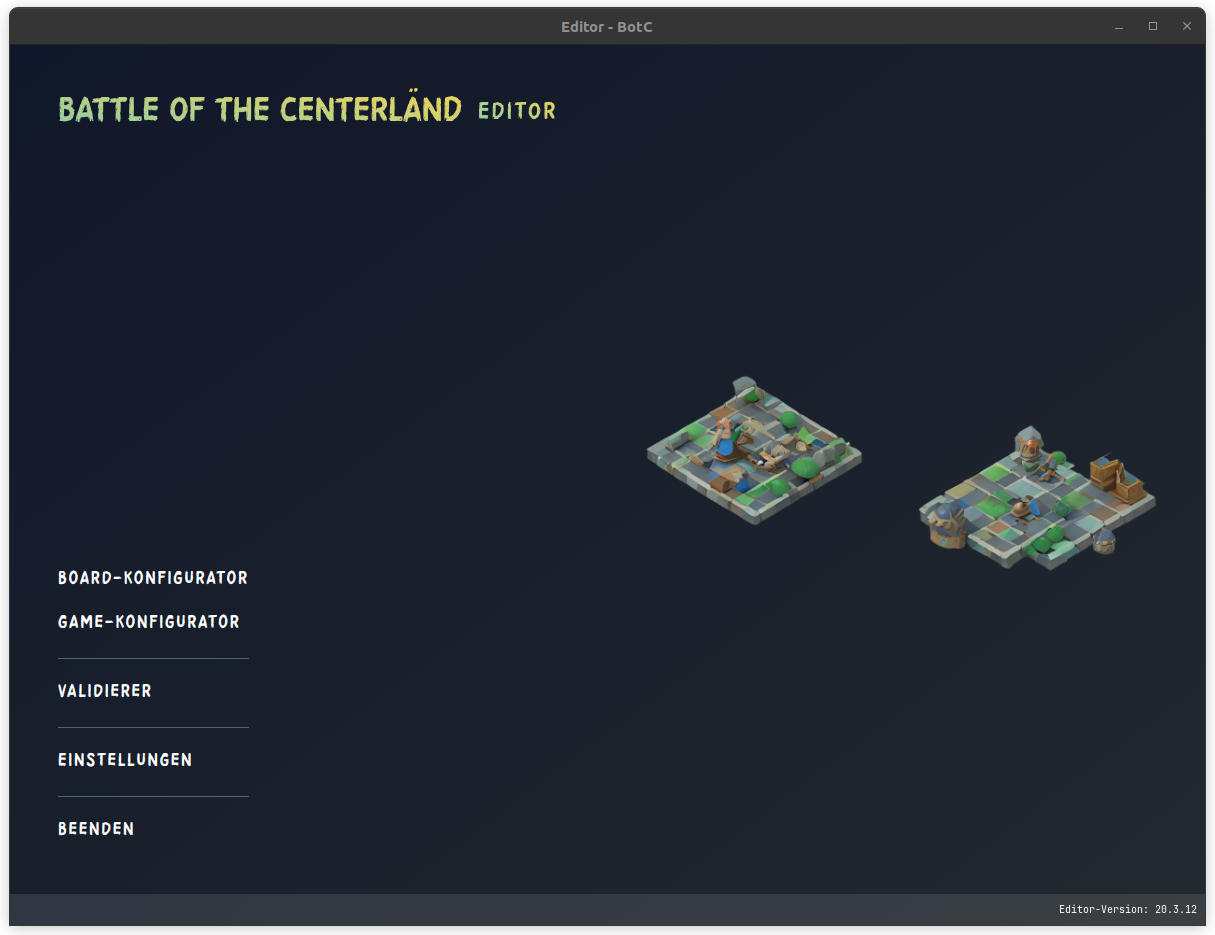
\includegraphics[width=\textwidth]{./Handbuch/assets/Startbildschirm}

Nach dem Start des Editors wird der Startbildschirm angezeigt.
Auf dem Startbildschirm kann der Benutzer auswählen, welche Komponente des Editors er starten möchte.
\\\\
Der Benutzer kann zwischen dem \emph{Board-Konfigurator}, dem \emph{Game-Konfigurator} und dem \emph{Validierer} wählen.
Außerdem kann der Benutzer unter \emph{Einstellungen} die Sprache des Editors ändern, das Design des Editors ändern und entscheiden, ob Popups bewegt werden können.
Über den Button \emph{Beenden} kann der Editor beendet werden.

\subsection{Board-Konfigurator}\label{subsec:board-konfigurator}

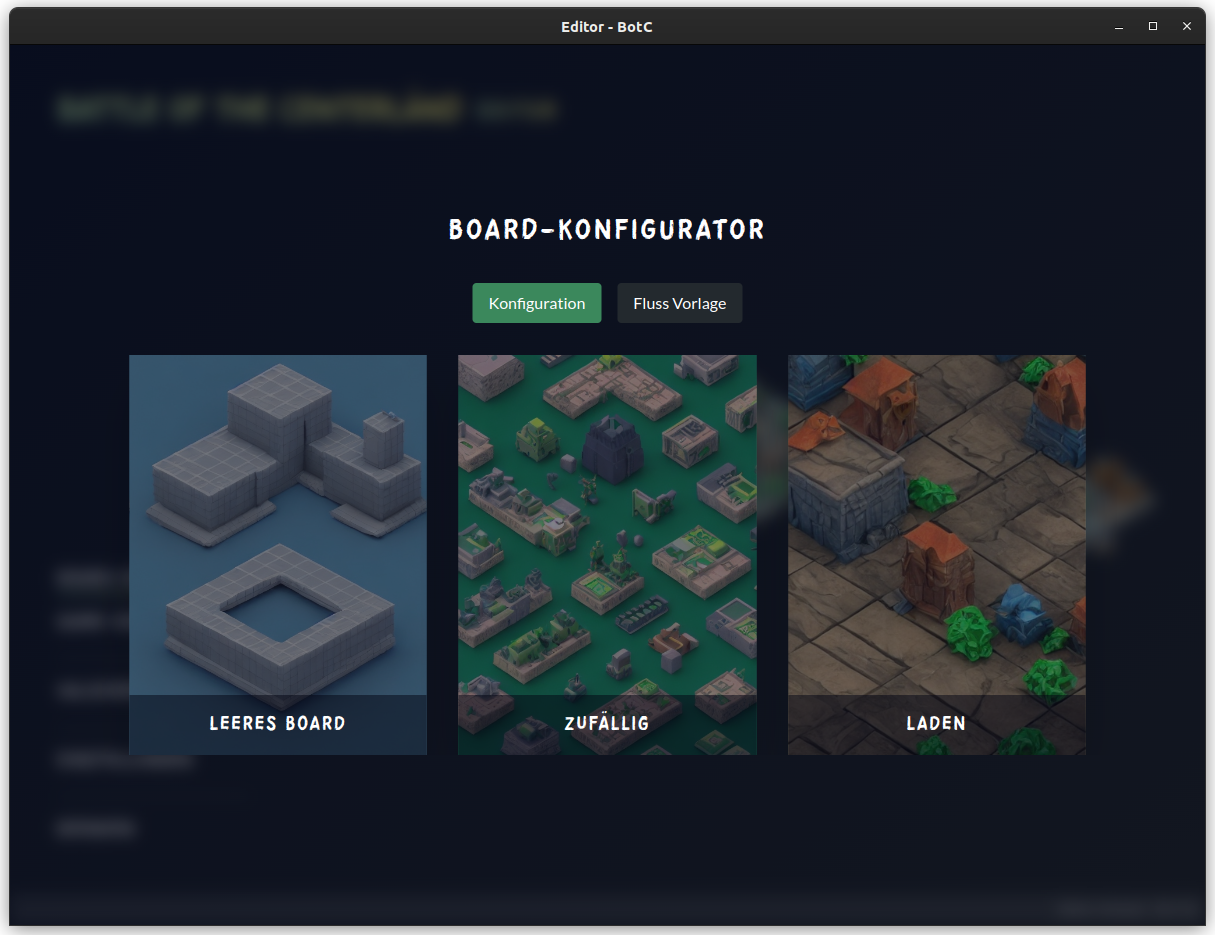
\includegraphics[width=\textwidth]{./Handbuch/assets/Board-Konfigurator-Choice}

Nachdem der Benutzer den \emph{Board-Konfigurator} gestartet hat, kann der Benutzer sich entscheiden, ob er ein neues Spielbrett erstellen möchte, ein Spielbrett laden möchte oder ein Spielbrett zufällig generieren möchte.

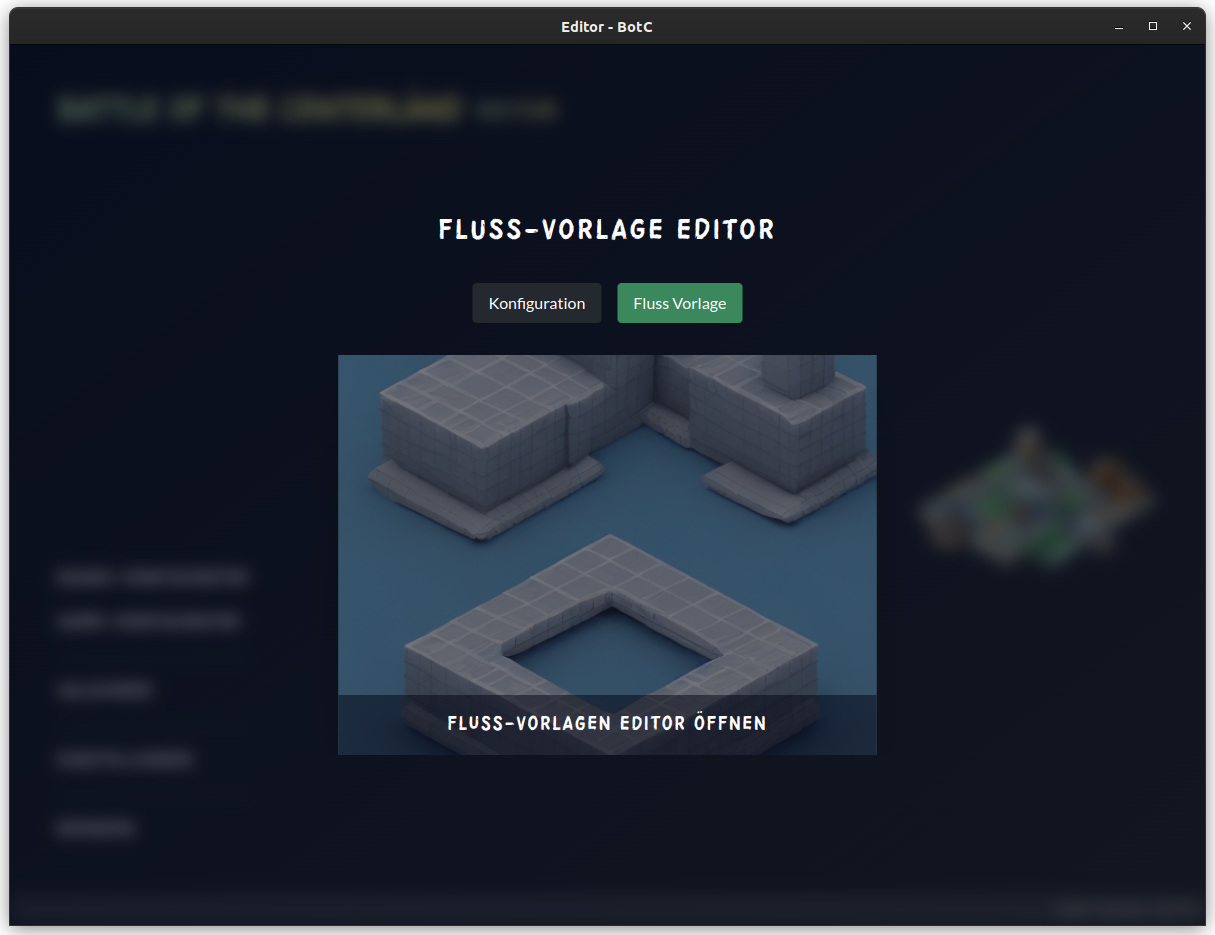
\includegraphics[width=\textwidth]{./Handbuch/assets/Board-Konfigurator-Choice-River-Presets}

Durch das Umschalten auf den Reiter \emph{Fluss Vorlage} kann der Benutzer den \emph{Fluss-Vorlagen Editor} starten.
Der \emph{Fluss-Vorlagen Editor} ermöglicht es dem Benutzer, Fluss-Vorlagen zu erstellen, zu bearbeiten und zu löschen.


\end{document}
